\section{Deployment diagram}
\vspace{0.5cm}

\begin{figure}[H]
    \centering
    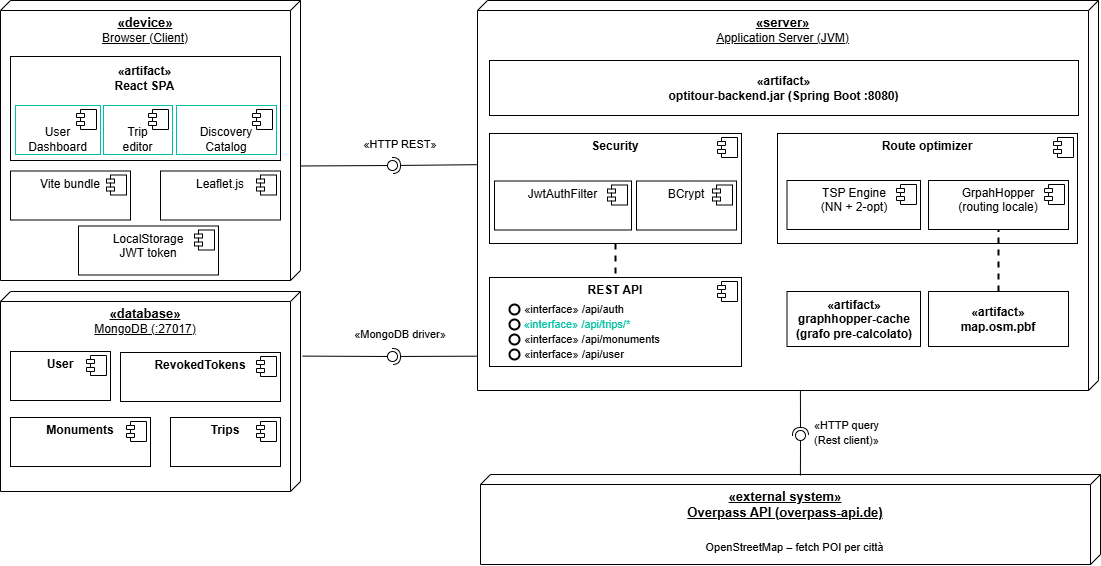
\includegraphics[width=0.85\textwidth]{Iterazione2/Diagrammi/DeploymentDiagram2.png}
    \caption{Diagramma di deployment}
    \label{fig:class_diagram2}
\end{figure}

Il diagramma di deployment è stato aggiornato per rappresentare le evoluzioni architetturali necessarie a supportare i nuovi casi d’uso dell’applicazione.\\
Come mostrato nel diagramma, tali modifiche non hanno richiesto l’introduzione di nuovi nodi fisici o di ulteriori database, ma hanno comportato un ampliamento dei moduli logici già presenti negli artefatti esistenti.

Per quanto riguarda l’interazione con l’utente, all’interno dell’artefatto \texttt{React SPA}, collocato nel nodo \textit{Browser (Client)}, sono stati definiti tre nuovi macro-componenti software che raccolgono la logica applicativa relativa ai seguenti Use Case (UC):

\begin{itemize}
    \item \textbf{User Dashboard}: gestisce l’area personale dell’utente e il monitoraggio dei suoi itinerari. Include i casi d’uso relativi alle preferenze e allo stato dei percorsi, ovvero \textit{UC3.3 (Visualizza storico)}, \textit{UC5 (Salva percorso nei preferiti)}, \textit{UC7 (Rimuovi percorso salvato)} e \textit{UC10 (Imposta percorso completato)}.

    \item \textbf{Trip editor}: modulo dedicato alla modifica degli itinerari esistenti. Implementa le funzionalità richieste dall’utente per aggiornare o rimuovere tappe, in particolare \textit{UC15 (Modifica tappe)} e \textit{UC16 (Elimina tappa)}.

    \item \textbf{Discovery Catalog}: componente orientato alla consultazione e alla scoperta di nuovi percorsi. Fornisce l’interfaccia per il catalogo pubblico (\textit{UC3.1 Visualizza catalogo}, \textit{UC8 Pubblica percorso nel catalogo}), per i filtri di ricerca (\textit{UC4 Filtri ricerca}) e per la generazione di itinerari casuali (\textit{UC12.2 Creazione itinerario casuale}).
\end{itemize}

Dal lato server, nel nodo \textit{Application Server (JVM)}, l’integrazione di queste funzionalità ha richiesto un’estensione dell’interfaccia \textbf{REST API}.\\
Nel diagramma, l’endpoint principale è stato generalizzato come \texttt{«interface» /api/trips/*} per indicare in modo formale l’esposizione dei nuovi sotto-percorsi (ad esempio: \texttt{/history}, \texttt{/catalog}, \texttt{/random}, \texttt{/\{id\}/save}) necessari a gestire le richieste HTTP provenienti dai moduli frontend introdotti.

\vspace{0.5cm}
